\documentclass[11pt,a4paper]{article}
\usepackage[margin=19mm,headheight=15pt]{geometry}
\usepackage[T1]{fontenc}
\usepackage{lmodern,microtype,amsmath,amssymb,booktabs,tabularx,graphicx}
\usepackage{caption,float,fancyhdr}
\usepackage[hidelinks]{hyperref}
\setlength{\parindent}{0pt}\setlength{\parskip}{5pt}
\setlength{\emergencystretch}{2em}
\captionsetup{font=small,labelfont=bf}
\pagestyle{fancy}\fancyhf{}
\fancyhead[L]{\small CSE 516: Probabilistic Graphical Models}
\fancyhead[R]{\small Group 4}\fancyfoot[C]{\thepage}
\newcommand{\N}{\mathcal N}
\begin{document}
\begin{titlepage}
\thispagestyle{empty}
\begin{center}
\vspace*{17mm}
{\Large\bfseries Ahmedabad University}\par\vspace{3mm}
{\Large\bfseries CSE 516 -- Probabilistic Graphical Models}\par\vspace{6mm}
{\large Milestone 4: Final Project Report}\par\vspace{17mm}
{\fontsize{18}{22}\selectfont\bfseries Bayesian Personalized Recommendation using\\[3pt]
Latent Trait Models \& Expectation Propagation}\par\vspace{7mm}
{\large Theoretical AI \quad | \quad Group 4}\par\vspace{13mm}
\renewcommand{\arraystretch}{1.2}
\begin{tabular}{ll}\toprule
\textbf{AU ID}&\textbf{Student Name}\\\midrule
AU2440170 & Jyotier Vithalani\\
AU2440234 & Tanmay Kanani\\
AU2440259 & Ansh Chaudhari\\
AU2440178 & Shlok Shah\\
AU2440221 & Het Patel\\\bottomrule
\end{tabular}
\vfill
\textbf{GitHub repository}\par
{\small\url{https://github.com/Jyotier2006/M2_g4_th_apl_recommend-sys_team}}\par\vspace{10mm}
\textbf{Submission date:} 12 November 2026
\end{center}
\end{titlepage}
\setcounter{page}{1}

\section*{Abstract}
A movie recommender should estimate both a rating and its uncertainty. We
compare single-pass assumed-density filtering (ADF), repeated expectation
propagation (EP), and matrix factorization with and without a Gaussian
Markov random field (GMRF) movie prior fitted by maximum a posteriori
(MAP) estimation. On five MovieLens 1M splits,
expected-rating RMSE decreases from $0.8977\pm0.0035$ for ADF to
$0.8548\pm0.0029$ for EP10. GMRF-MAP reaches $0.8499\pm0.0023$, versus
$0.8506\pm0.0021$ for graph-free MAP. The isolated graph gain is small on
clean data and larger when ratings are removed or corrupted. EP improves
log-loss but worsens calibration error. Numerical reference checks and a
fresh run of split 42 check the implementation and reported scores.

\section{Introduction}
A user typically rates only a small part of the movie catalogue. Latent
traits let ratings inform other user--movie pairs, while a probability
distribution distinguishes confident predictions from uncertain ones.

\subsection{Problem Formulation}
Given training ratings $\mathcal D_{\rm train}$, estimate
$p(R_{ui}=r\mid\mathcal D_{\rm train})$ for a held-out pair $(u,i)$ and
$r\in\{1,\ldots,5\}$. We test whether repeated inference passes improve
prediction and whether a movie graph helps when the fitting method is fixed.

MovieLens 1M contains 1,000,209 ratings from 6,040 users on 3,706 rated movies,
or 4.47\% of possible pairs~\cite{movielens,harper2015}. User and movie IDs
index parameter arrays; star ratings are observations. Movie genres form
18 binary features for graph construction. Timestamps and user demographics
are audited but not used as predictors. Missing ratings are not zeros.

\section{Background}
Latent factor models represent user preferences and movie properties as
vectors. A dot product measures affinity, and an ordinal likelihood maps
a noisy score to ordered stars. EP approximates the resulting posterior
with Gaussian beliefs; MAP instead estimates one parameter setting.

\subsection{Related Work}
\textbf{Microsoft Research Matchbox.}
Stern, Herbrich and Graepel~\cite{stern2009} map user and item features into
Gaussian traits and combine EP with variational message passing (VMP).
Their system supports metadata, user-specific ordinal scales and dynamics.
On MovieLens and Netflix they demonstrate practical single-pass ADF and
gains from additional EP passes. We retain the trait product and hybrid
updates in a static, ID-only ordinal model with global thresholds.

\textbf{Research anchor: PreRec.} Lin et al.~\cite{lin2024} use a hierarchical
Bayesian model with neural user and item encoders, domain and popularity
variables, and MAP training. Their cross-market and cross-platform
experiments study zero- and few-shot ranking using Recall and revised NDCG.
\subsection{SOTA Positioning}
Matchbox provides the inference design for the ADF--EP comparison. PreRec
illustrates how structured priors can share sparse evidence across domains.
We test a fixed movie graph within one dataset. The published system scores
are not directly comparable with our held-out rating scores.

\clearpage
\section{Graphical Representation}
\subsection{Ordinal latent traits}
For user $u$ and movie $i$, let $s_u,t_i\in\mathbb R^K$ be latent traits
and $b_u,b_i$ scalar biases. Affinity $a_{ui}$ generates a noisy score
$y_{ui}$ and then a star rating:
\begin{align}
a_{ui}&=\mu+b_u+b_i+s_u^Tt_i, & y_{ui}\mid a_{ui}&\sim\N(a_{ui},\beta^2),\\
R_{ui}=r&\iff c_{r-1}<y_{ui}\le c_r,&
c&=(-\infty,1.5,2.5,3.5,4.5,\infty).
\end{align}
The offset $\mu$ is the training mean. Biases have independent $\N(0,1)$
priors; traits have variance $0.25$ and small seeded prior means.
With $\theta=(s,t,b)$, the factorization is
$p(\theta,R)=p(\theta)\prod_{(u,i)\in\mathcal D}p(R_{ui}\mid a_{ui})$,
where each star likelihood is the Gaussian mass between adjacent cuts.
Ratings are independent given the relevant traits and biases. Shared
parameters create dependence after marginalization. Factorization of the
\emph{approximate posterior} is a separate computational assumption.

\begin{figure}[H]\centering
\begin{minipage}[c]{.49\linewidth}\centering
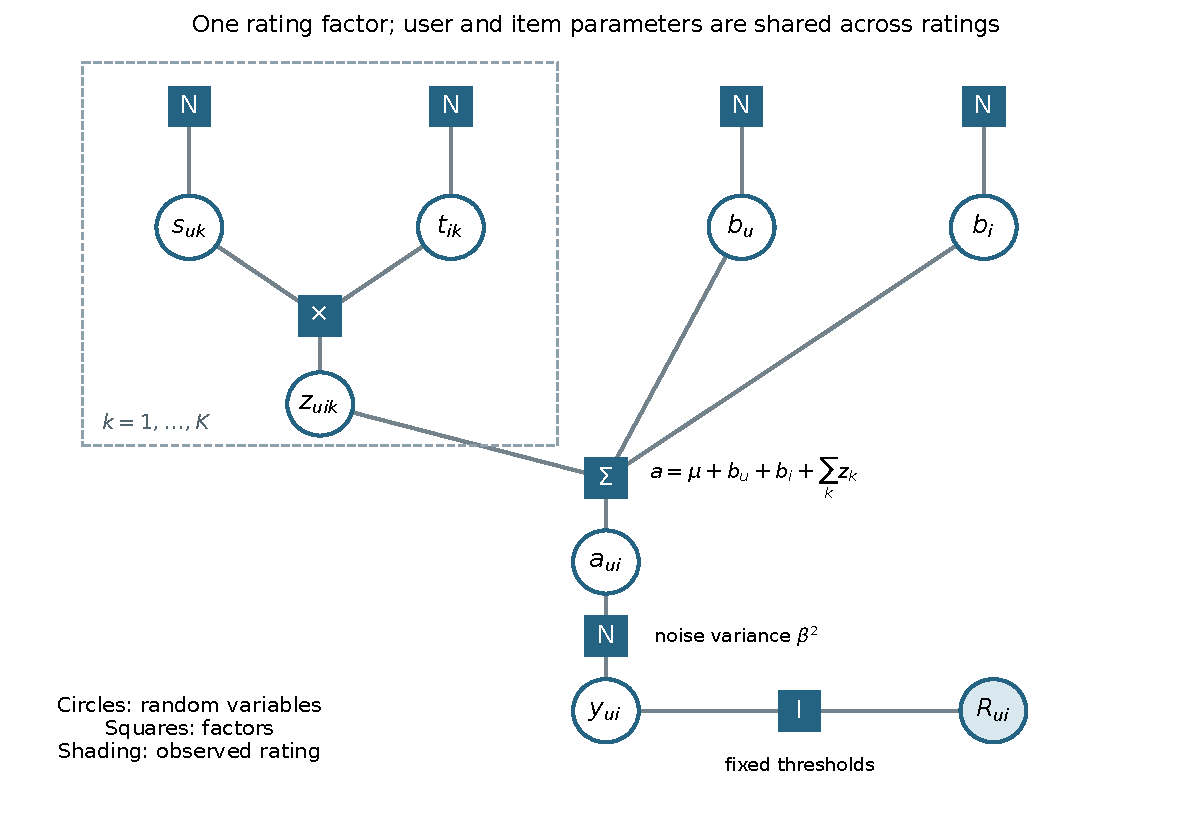
\includegraphics[width=\linewidth]{figures/factor_graph.pdf}\par
{\small (a) Ordinal rating factor graph}
\end{minipage}\hfill
\begin{minipage}[c]{.49\linewidth}\centering
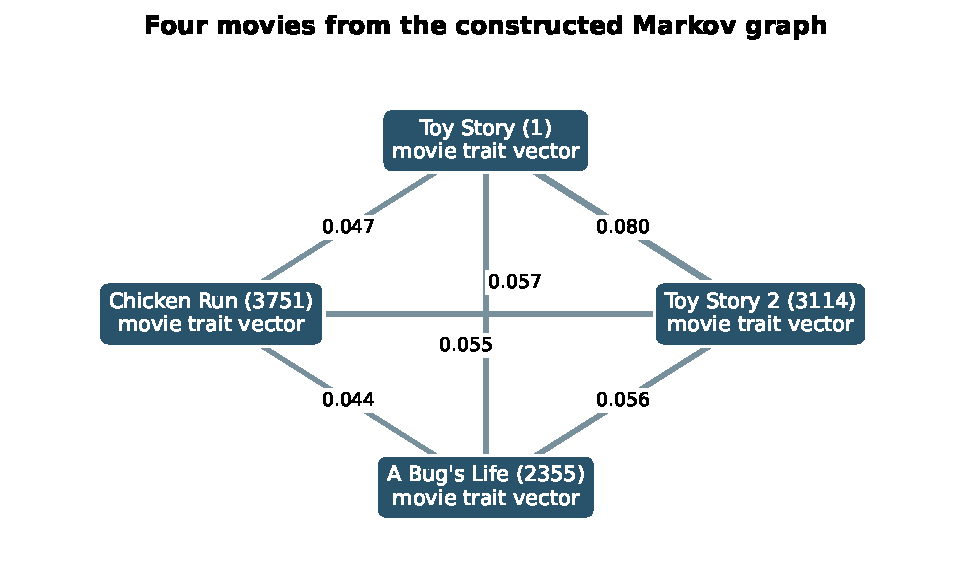
\includegraphics[width=\linewidth]{figures/movie_subgraph.pdf}\par
{\small (b) Movie prior subgraph, seed 42}
\end{minipage}
\caption{Circle nodes in (a) are variables; squares compute products,
sums, noise and thresholding. Edges in (b) couple movie vectors with the
displayed normalized weights.}
\end{figure}

\subsection{Gaussian Markov movie prior}
We build a graph using positive cosine similarity of training residuals
after removing fitted user/movie biases. Similarities require five
co-raters and are shrunk by $n_{ij}/(n_{ij}+20)$. The default score mixes
90\% residual similarity with 10\% genre similarity. Keep the 20 strongest
positive neighbours per movie, symmetrize by maximum weight, then normalize
the symmetric affinity by both endpoint degrees. The resulting weights $W$
define $D_{ii}=\sum_j W_{ij}$ and $L=D-W$. Validation and test ratings never
enter this construction. It estimates a fixed similarity graph, not a
causal structure or a posterior over graphs.

For each movie trait coordinate the precision is $J=\lambda I+\gamma L$.
Equivalently, the prior over movie vectors $Q$ is
\[
p(Q\mid W)\propto
\prod_i e^{-\lambda\|Q_i\|^2/2}
\prod_{\{i,j\}\in E}e^{-\gamma w_{ij}\|Q_i-Q_j\|^2/2}.
\]
The edge penalty shares evidence by pulling neighbouring traits together.
For $\lambda>0$ and $\gamma\ge0$, $J$ is positive definite (Appendix~A).
A zero off-diagonal entry means conditional independence given the other
movie traits in the prior, not marginal independence.

\clearpage
\section{Learning Method}
\subsection{Bayesian parameter learning with ADF and EP}
Bilinear products and ordinal observations couple many unknowns, so exact
posterior inference is not practical at this scale. We approximate each
scalar belief by a Gaussian. Precision and weighted mean, $\lambda=1/v$
and $\eta=m/v$, add when Gaussian factors are multiplied. EP stores a
rating's contribution as a site. To revisit rating $n$, it first removes
that contribution:
\[
(\lambda^{\setminus n},\eta^{\setminus n})=(\lambda-\lambda_n,\eta-\eta_n).
\]
The observed rating restricts the score to its star interval. EP matches
the truncated score's mean and variance and divides out its incoming
Gaussian. VMP passes the resulting information through each product using
the partner's first and second moments. The site is replaced with damping
and added back. ADF visits each rating once and discards its site; the first
EP pass is therefore identical to ADF under the same initialization and
order. EP5 and EP10 revisit the same data, not new ratings. Default outer
damping is 1 for the first pass and 0.5 thereafter; local damping is 0.7
with a ten-iteration cap and $10^{-4}$ tolerance.

\subsection{Graph-regularized MAP}
The MAP model uses score $f_{ui}=\mu+b_u+b_i+P_u^TQ_i$ and a unit-variance
Gaussian training likelihood for numeric ratings. It minimizes
\[
\mathcal E=\tfrac12\sum_{\mathcal D}(R_{ui}-f_{ui})^2+
\tfrac\lambda2(\|P\|_F^2+\|Q\|_F^2)+
\tfrac{\lambda_b}2(\|b_U\|^2+\|b_I\|^2)+
\tfrac\gamma2\operatorname{tr}(Q^TLQ).
\]
Alternating exact block solves update a user or movie vector together with
its bias. Neighbours affect the movie solve through both its precision and
weighted target (Appendix~A). Each block decreases or preserves the energy;
joint optimization is nonconvex. Setting $\gamma=0$ removes graph smoothing
while retaining the same likelihood, base penalties and block solver.

\section{Inference Method}
For independent Gaussian traits $s_k,t_k$ in the approximate posterior,
the product has mean $m_{s_k}m_{t_k}$ and variance
$v_{s_k}v_{t_k}+v_{s_k}m_{t_k}^2+v_{t_k}m_{s_k}^2$. Sum these moments with
the biases and observation noise to obtain $m_y,v_y$. A Gaussian
approximation for the total score gives
\[
p_r=\Phi\left(\frac{c_r-m_y}{\sqrt{v_y}}\right)-
\Phi\left(\frac{c_{r-1}-m_y}{\sqrt{v_y}}\right),\qquad
\hat r=\sum_{r=1}^5 r p_r.
\]
Expected stars are used for RMSE and MAE; the modal star is used for exact
accuracy. The calculation uses the fitted marginal variances and omits
posterior covariances.

For MAP, use $m_y=f_{ui}$ and a residual variance $v_y$ selected by
validation log-loss. This yields probabilities over the same star bins
without integrating uncertainty over model parameters.

\textbf{Complexity.} For $N$ observations, $K$ traits, $H$ local iterations
and $T$ passes, EP fitting costs $O(TNH(K+1))$. Its sites require
$32N(K+1)$ bytes: 219.77 MiB at $K=8$ here. ADF retains no sites. Batch
prediction costs $O(N(K+1))$. MAP costs
$O(T[N(K+1)^2+(U+I)(K+1)^3+|E|K])$ plus graph construction, with sparse
graph storage $O(|E|)$. No convergence guarantee is inferred from finite runs.

\clearpage
\section{Experimental Setup}
Seeds 42--46 each give 800,167 train, 100,020 validation and 100,022 test
ratings. Methods share the same split within a seed and use expected stars
for point error. The ordinal models use $K=8$ and default $\beta^2=1$.
MAP uses $\lambda=\lambda_b=10$, up to 25 epochs and
$\gamma\in\{0,1,10,100\}$. Validation clipped RMSE selects checkpoints and
graph strength; validation log-loss selects the residual variance. Test
ratings are used only for evaluation.

\subsection{Baselines}
Global uses the training star frequencies. User and item means use the
corresponding frequencies smoothed toward the global distribution. MF-SGD
fits eight traits by stochastic gradient descent (25 epochs, learning
rate 0.007, decay 0.98, regularization 0.03). ADF is the single-pass
control for EP; MF-MAP at $\gamma=0$ isolates the effect of the graph.

\subsection{KPIs}
\textbf{Representation:} parameter count, graph size, mean degree and
density. No reference graph exists for structural recovery metrics.

\textbf{Inference:} RMSE is the square root of the mean squared star error;
MAE averages absolute star error. Negative log-likelihood
$-N^{-1}\sum_n\log p_{n,R_n}$ equals categorical log-loss. Brier averages
$\sum_r(p_{nr}-\mathbf1\{r=R_n\})^2$. Expected calibration error (ECE)
compares confidence and accuracy across ten bins. Star accuracy measures
how often the modal star is correct. Prediction time is measured per batch.

\textbf{Learning:} fitting time, validation RMSE over EP passes, and the
MAP objective over epochs.

\section{Results}
The models have $(6040+3706)(8+1)=87,714$ scalar traits and biases.
The movie graph has 3,706 nodes, $56,508\pm69$ edges, mean degree 30.50,
density 0.823\%, and no isolated nodes on the five main splits.

\begin{table}[H]\centering\footnotesize
\begin{tabular}{@{}lrrrrr@{}}\toprule
Method & RMSE & NLL & Brier & ECE & Stars (\%)\\\midrule
Global & 1.1164 $\pm$ 0.0021 & 1.4552 $\pm$ 0.0015 & 0.7440 $\pm$ 0.0005 & 0.0008 $\pm$ 0.0006 & 34.91 $\pm$ 0.08\\
User mean & 1.0342 $\pm$ 0.0021 & 1.3461 $\pm$ 0.0016 & 0.7022 $\pm$ 0.0006 & 0.0059 $\pm$ 0.0015 & 39.67 $\pm$ 0.12\\
Item mean & 0.9786 $\pm$ 0.0026 & 1.3209 $\pm$ 0.0028 & 0.6952 $\pm$ 0.0010 & 0.0054 $\pm$ 0.0027 & 40.58 $\pm$ 0.08\\
MF-SGD & 0.8683 $\pm$ 0.0024 & 1.2214 $\pm$ 0.0025 & 0.6554 $\pm$ 0.0011 & 0.0397 $\pm$ 0.0010 & 46.04 $\pm$ 0.16\\
ADF / EP1 & 0.8977 $\pm$ 0.0035 & 1.2519 $\pm$ 0.0033 & 0.6681 $\pm$ 0.0012 & 0.0451 $\pm$ 0.0010 & 44.13 $\pm$ 0.13\\
EP3 & 0.8740 $\pm$ 0.0036 & 1.2283 $\pm$ 0.0033 & 0.6590 $\pm$ 0.0012 & 0.0537 $\pm$ 0.0017 & 45.20 $\pm$ 0.18\\
EP5 & 0.8643 $\pm$ 0.0037 & 1.2189 $\pm$ 0.0035 & 0.6552 $\pm$ 0.0012 & 0.0566 $\pm$ 0.0009 & 45.59 $\pm$ 0.16\\
EP10 & 0.8548 $\pm$ 0.0029 & 1.2098 $\pm$ 0.0024 & 0.6516 $\pm$ 0.0007 & 0.0608 $\pm$ 0.0012 & 46.04 $\pm$ 0.21\\
MF-MAP & 0.8506 $\pm$ 0.0021 & 1.2012 $\pm$ 0.0021 & 0.6467 $\pm$ 0.0007 & 0.0383 $\pm$ 0.0018 & 46.98 $\pm$ 0.15\\
GMRF-MAP & 0.8499 $\pm$ 0.0023 & 1.2007 $\pm$ 0.0024 & 0.6468 $\pm$ 0.0009 & 0.0387 $\pm$ 0.0022 & 46.96 $\pm$ 0.19\\
\bottomrule\end{tabular}

\caption{MovieLens 1M test results, mean $\pm$ sample SD across five splits.}
\end{table}
EP5 reduces ADF RMSE by about 0.0334 stars; EP10 improves it further.
MF-SGD is a strong low-cost baseline. GMRF-MAP has the best mean RMSE,
but graph-free MF-MAP is close and has slightly better star accuracy and
ECE. The comparison between EP and MAP changes the likelihood and
estimator as well as the prior. The matched MAP comparison isolates
graph smoothing.

\clearpage
\subsection{Cost, Calibration and Error Analysis}
\begin{table}[H]\centering\small
\begin{tabular}{@{}lrrr@{}}\toprule
Method & Fit (s) & Predict (ms / 1000) & MAE\\\midrule
MF-SGD & 1.38 $\pm$ 0.04 & 0.413 $\pm$ 0.014 & 0.6906 $\pm$ 0.0023\\
ADF / EP1 & 3.33 $\pm$ 0.19 & 0.810 $\pm$ 0.143 & 0.7098 $\pm$ 0.0030\\
EP5 & 18.29 $\pm$ 2.02 & 0.679 $\pm$ 0.088 & 0.6808 $\pm$ 0.0025\\
EP10 & 35.99 $\pm$ 6.61 & 0.779 $\pm$ 0.298 & 0.6721 $\pm$ 0.0018\\
MF-MAP & 16.74 $\pm$ 2.74 & 0.449 $\pm$ 0.060 & 0.6753 $\pm$ 0.0017\\
GMRF-MAP & 14.48 $\pm$ 1.82 & 0.487 $\pm$ 0.096 & 0.6752 $\pm$ 0.0019\\
\bottomrule\end{tabular}

\caption{Mean $\pm$ SD of preserved five-split timings and MAE.
Fit times exclude JIT warm-up; prediction times are batch measurements.}
\end{table}
EP5 takes about 5.5 times as long to fit as ADF. The selected GMRF
candidate takes 14.48 s on average; building the graph takes 4.31 s and
the full four-candidate search takes 66.37 s, including the selected
candidate. Candidate time alone is not total workflow cost. The
validation traces show improving EP error over passes and nonincreasing
MAP energy. EP's mean RMS parameter change at pass 10 is still 0.01564.

\begin{figure}[H]\centering
\begin{minipage}[c]{.51\linewidth}\centering
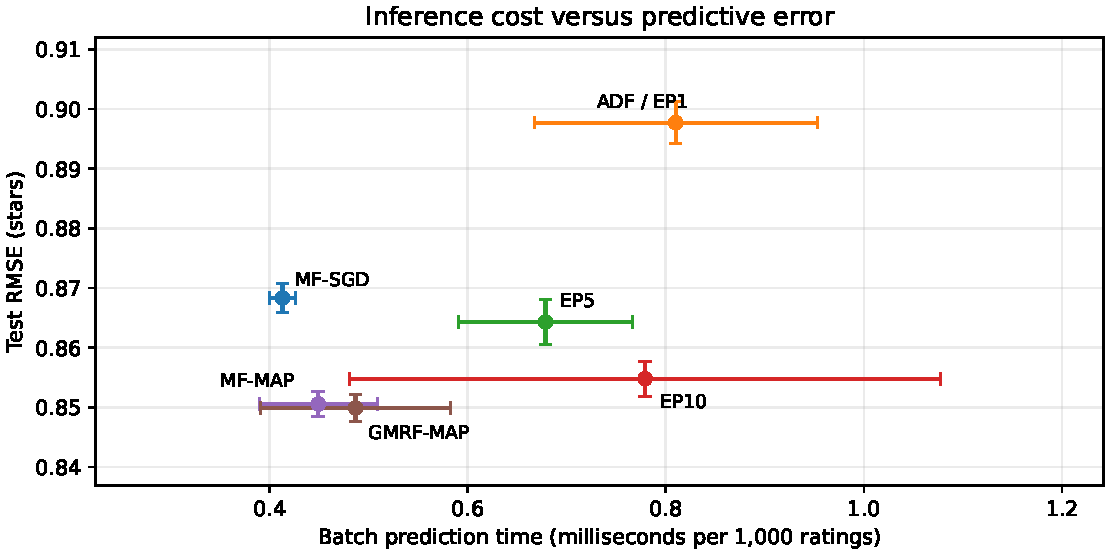
\includegraphics[width=\linewidth]{figures/inference_tradeoff.pdf}
\end{minipage}\hfill
\begin{minipage}[c]{.47\linewidth}\centering
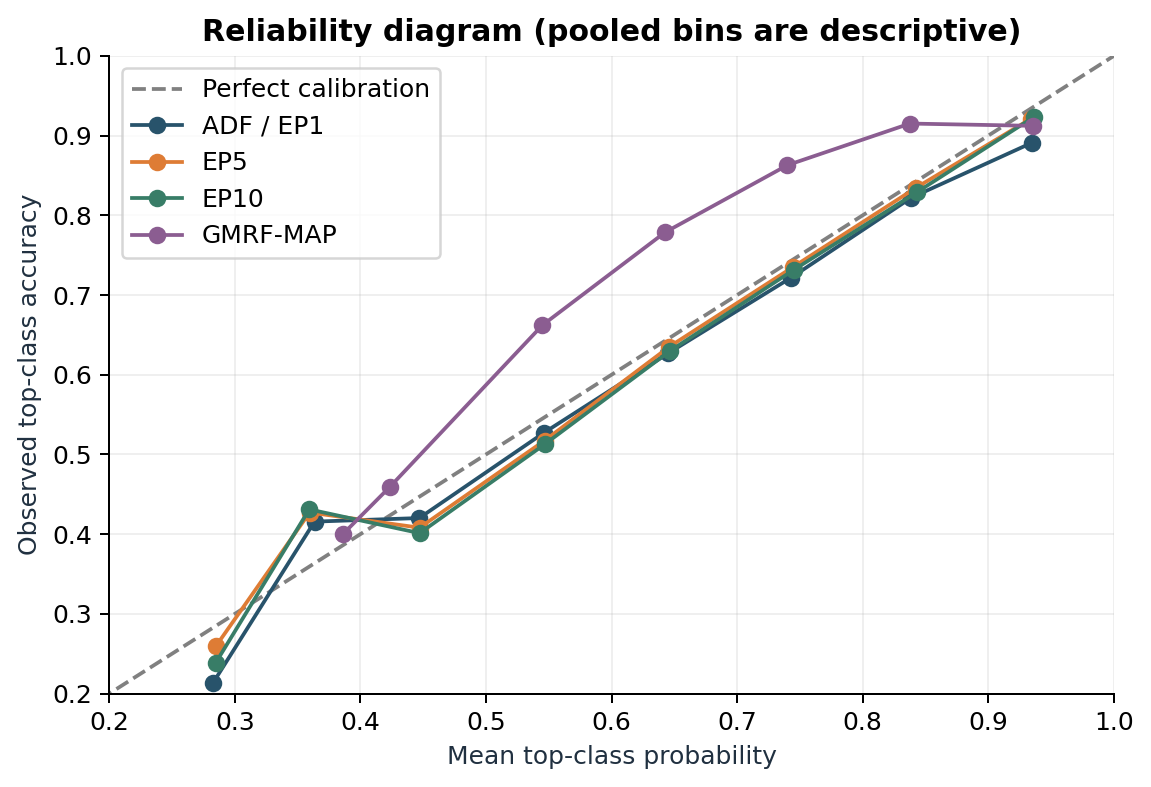
\includegraphics[width=\linewidth]{figures/reliability.png}
\end{minipage}
\caption{Batch prediction time versus RMSE (left, mean $\pm$ SD) and
top-class reliability (right, pooled descriptively across overlapping splits).}
\end{figure}
EP improves log-loss and Brier over ADF while ECE rises from 0.0451 to
0.0608 at EP10. Observation variance 1 wins every EP5 validation log-loss
comparison; using 0.5 lowers ECE to 0.0339 but worsens RMSE to 0.8691 and
log-loss to 1.2404. This assumption test differs from corrupting ratings.
At damping 1, EP5 reaches 0.8529 on the three sensitivity seeds, versus
0.8633 at default damping. Tuning the update schedule can close much of
the gap to MAP; this exploratory result does not replace the main method.

Errors are largest on low-support items and extreme ratings. For observed
five-star ratings, GMRF RMSE is 1.0245 versus 0.9748 for EP10 despite its
better aggregate RMSE. The expected-star decision and regularization
shrink predictions towards the centre. Nominal 90\% EP5 intervals cover
98.22\% but span 3.82 star categories on average; high coverage alone
does not establish good calibration.

\clearpage
\section{Statistical Analysis}
All five validation splits choose $\gamma=10$. Mean graph-only RMSE
reduction is 0.000644 stars (0.076\%). Within each split we resample users
with replacement 2,000 times, keeping each user's test ratings paired
across methods. Percentile 95\% intervals are conditional on the fitted
models and omit retraining and shared-item dependence. Four graph-effect
intervals exclude zero and one includes it. This is conditional evidence
of a small effect, not an independent-replication significance claim.
The five splits overlap, so we do not use a paired t-test treating them
as independent observations.

\begin{figure}[H]\centering
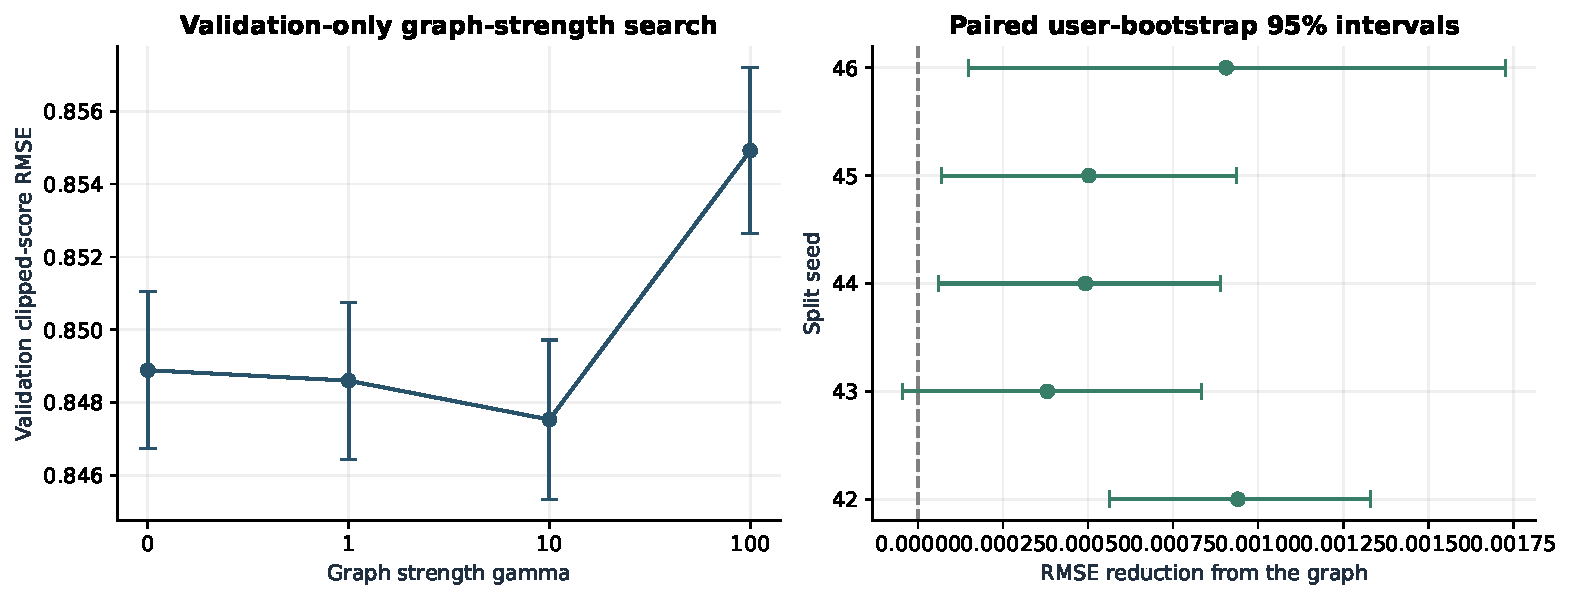
\includegraphics[width=\linewidth]{figures/graph_evidence.pdf}
\caption{Validation graph-strength search and paired 95\% intervals.
Positive differences favour the graph. Strength 100 worsens validation error.}
\end{figure}

\subsection{Robustness and Ablation}
\begin{table}[H]\centering\footnotesize
\begin{tabular}{@{}lrrrr@{}}\toprule
Condition & ADF & EP5 & MF-MAP & GMRF-MAP\\\midrule
main & 0.8980 $\pm$ 0.0049 & 0.8633 $\pm$ 0.0040 & 0.8507 $\pm$ 0.0028 & 0.8501 $\pm$ 0.0031\\
retain\_0.25 & 0.9217 $\pm$ 0.0041 & 0.9199 $\pm$ 0.0051 & 0.9178 $\pm$ 0.0042 & 0.9100 $\pm$ 0.0038\\
retain\_0.5 & 0.9102 $\pm$ 0.0039 & 0.8920 $\pm$ 0.0049 & 0.8810 $\pm$ 0.0039 & 0.8775 $\pm$ 0.0041\\
noise\_0.1 & 0.9129 $\pm$ 0.0036 & 0.8910 $\pm$ 0.0036 & 0.8827 $\pm$ 0.0029 & 0.8797 $\pm$ 0.0030\\
noise\_0.2 & 0.9386 $\pm$ 0.0030 & 0.9326 $\pm$ 0.0022 & 0.9317 $\pm$ 0.0023 & 0.9248 $\pm$ 0.0018\\
cold\_items & 1.0703 $\pm$ 0.0079 & 1.0781 $\pm$ 0.0068 & 1.0622 $\pm$ 0.0060 & 1.0545 $\pm$ 0.0077\\
cold\_users & 0.9837 $\pm$ 0.0137 & 0.9861 $\pm$ 0.0146 & 0.9935 $\pm$ 0.0115 & 0.9916 $\pm$ 0.0117\\
\bottomrule\end{tabular}

\caption{Three-seed stress tests, mean $\pm$ SD. Cold-start rows use
restricted test populations, so compare methods within each row.}
\end{table}
We retain nested 25\%/50\% training subsets, or change 10\%/20\% of
training labels to another star. Validation/test labels stay clean.
Graphs are rebuilt from each condition; strength 10 is fixed, with
validation still selecting epochs. The graph gain grows to 0.0077 RMSE
at 25\% retention and 0.0069 with 20\% corruption. Smoothing mitigates
some damage without restoring clean-data performance.

Holding out all training rows for 10\% of movie IDs tests cold movies;
genre links remain available. The graph improves 1.0622 to 1.0545 RMSE.
For a corresponding held-out user test, ADF beats GMRF (0.9837 versus
0.9916): movie links cannot infer an unseen user's taste. On clean
three-seed splits, rating-only edges work slightly better than mixed edges;
genre-only edges worsen RMSE versus no graph. Top-5 improves on top-50.
These are exploratory ablations, not test-driven changes to the main model.

\clearpage
\section{Discussion}\label{sec:discussion}
Repeated EP improves on ADF with the ordinal representation fixed. Later
passes reconsider each observation after other beliefs have changed, at
the cost of more memory and fitting time. This confirms a limited part of
Matchbox's inference trade-off under fixed thresholds and static traits.
It does not reproduce its online dynamics, personalized rating scales or
published system-level results.

PreRec's transferable encoders and causal mechanisms target a different
setting. Our experiments validate a narrower idea: sharing information
through a fixed prior can help when evidence is thin. The matched
$\gamma=0$ ablation shows only a modest clean-data benefit; genre-only
links and unseen users expose its limits. We therefore position the work
as a reproducible study of approximate inference and graph regularization,
not a new state-of-the-art recommender or a reproduction of PreRec.

\section{Limitations and Future Work}
Random-interaction splits do not represent future deployment. EP drops
posterior covariance, while MAP treats traits and graph weights as fixed
for prediction. Estimated edges can reflect exposure patterns rather than
preference similarity. Artificial missingness and noise do not capture
every real failure. Searches are finite, and confidence intervals hold
training fixed. A useful next experiment would use chronological splits
and compare posterior-aware graph inference with matched graph-free
inference, controlling model capacity and calibration on validation data.

\section{Conclusion}
Repeated EP improves point and probability scores over ADF at a clear
computational cost, without uniformly improving calibration. GMRF-MAP
achieves 0.8499 RMSE, but most of its gain over EP is also present in
graph-free MAP. Its isolated benefit is most useful with fewer or noisier
training ratings. A movie graph can help an unseen movie when metadata is
available; it cannot personalize a user with no observations.

\bibliographystyle{plain}
\bibliography{references}

\clearpage
\appendix
\section{Derivations and verification}
\textbf{Proper prior and movie update.}
For any nonzero $x$,
$x^TJx=\lambda\|x\|^2+\gamma\sum_{\{i,j\}}w_{ij}(x_i-x_j)^2>0$.
The conditional mean of movie trait $Q_{ik}$ given all other movie values
is $\gamma\sum_j w_{ij}Q_{jk}/(\lambda+\gamma D_{ii})$, and the
conditional variance is $(\lambda+\gamma D_{ii})^{-1}$.
For the MAP movie block $z=(Q_i,b_i)$, let $x_u=(P_u,1)$ and
$y_u=R_{ui}-\mu-b_u$. Setting the derivative to zero gives
\[
\left[\sum_{u\in\mathcal D_i}x_ux_u^T+
\operatorname{diag}\big((\lambda+\gamma D_{ii})I_K,\lambda_b\big)\right]z
=\sum_{u\in\mathcal D_i}x_u y_u+
\gamma\begin{pmatrix}\sum_j w_{ij}Q_j\\0\end{pmatrix}.
\]
This system is positive definite. Its unique minimizer cannot increase
the objective when the other blocks stay fixed.

\textbf{Ordinal moment matching.}
For incoming score $\N(m,v)$ and observed star $r$, set
$a=(c_{r-1}-m)/\sqrt v$, $b=(c_r-m)/\sqrt v$ and
$Z=\Phi(b)-\Phi(a)$. With standard normal density $\phi$, the tilted mean
and variance are
\[
m'=m+\sqrt v\frac{\phi(a)-\phi(b)}Z,\qquad
v'=v\left[1+\frac{a\phi(a)-b\phi(b)}Z-
\left(\frac{\phi(a)-\phi(b)}Z\right)^2\right].
\]
Subtract the incoming Gaussian natural parameters from $(1/v',m'/v')$
to obtain the outgoing message. This local calculation does not make
the entire bilinear posterior exact.

\textbf{Algorithmic validation.}
Nine implementation checks passed, including ADF--EP1 equality, site
bookkeeping, reference-kernel equivalence and nonincreasing MAP energy.
Independent 40/80-point quadrature agrees to $1.04\times10^{-10}$ in the
one-observation bilinear case. Hybrid inference underestimates the two
reference variances by about 10\% and omits a covariance of 0.0705.
In a 12-variable Gaussian reference, the exact mean is $J^{-1}h$ and
covariance $J^{-1}$. Gauss--Seidel mean RMSE falls from 0.138 at one
sweep to $4.46\times10^{-8}$ at 20 sweeps; Gibbs estimates variances
as well, with sampling error. These are tractable diagnostics, separate
from MovieLens prediction scores.

\textbf{Verification.}
A fresh full-data run on seed 42 reproduced 146 recorded metric and
selection values across 17 method rows within $10^{-8}$, excluding
timings. Split hashes matched. The recorded-results audit checked 229
comparison rows and the expected seed and condition coverage. See
\texttt{Code/README.md} for the exact commands, dependencies and seeds,
and \texttt{Results/} for raw tables, uncertainty intervals, logs and figures.

\textbf{Latent dimension.}
A separate three-seed EP5 experiment obtained RMSE of $0.8760\pm0.0059$
with two traits and $0.8633\pm0.0040$ with eight. These runs are separate
from the five-split benchmark.

\begin{figure}[H]\centering
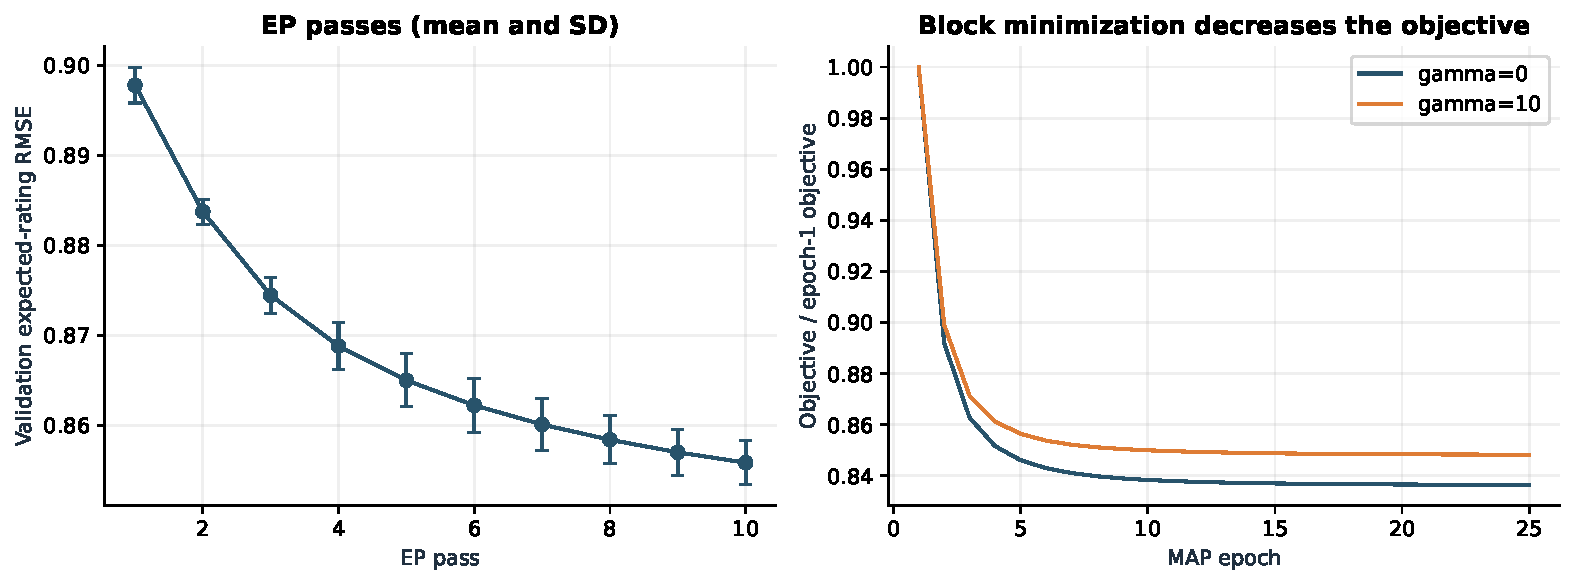
\includegraphics[width=.86\linewidth]{figures/convergence.pdf}
\caption{Learning traces: validation RMSE over EP passes and the normalized
MAP objective over epochs, averaged across the recorded splits.}
\end{figure}
\end{document}
